\section*{Introduction}


Scientific research serves as the cornerstone of human advancement, playing a crucial role in expanding knowledge, driving technological innovation, solving complex problems, enhancing education, improving societal welfare, fostering global collaboration, stimulating economic growth, and enriching cultural and intellectual life. It not only deepens our understanding of the natural world, technological possibilities, and social phenomena but also transforms economies through the creation and refinement of technologies, ultimately elevating quality of life and productivity across societies ~\cite{gibbons1974roles, sciencenoy2023experimental}. 


Despite its critical importance, the current landscape of academic research is characterized by inherent complexity and methodological constraints that frequently hinder rapid scientific advancement. Traditional research approaches necessitate labor-intensive processes, comprehensive literature analyses, and precise experimental design and execution, collectively consuming substantial time and resources ~\cite{rossoni2023barriers, vamathevan2019applications}. Furthermore, reliance on specialized expertise limits the progress and innovative capacity of research due to the dependence on a limited pool of experts ~\cite{Fabrykowska2020}. Cross-disciplinary knowledge integration serves as a pivotal factor in advancing research frontiers, particularly when addressing multifaceted global challenges in sustainable development and health sciences ~\cite{daniel2022challenges, freeth2020learning}. Multidisciplinary collaboration has yielded considerable benefits by synthesizing diverse expertise and perspectives, thus generating more comprehensive and innovative research outcomes ~\cite{toner2024artificial}. However, these collaborative efforts routinely encounter significant obstacles, including divergent disciplinary cultures ~\cite{daniel2022challenges}, specific methodologies~\cite{macleod2018makes}, and the considerable time and resources required to coordinate across fields. These persistent barriers undermine effective communication, conceptual synthesis, and the establishment of cohesive research paradigms.

Recent advancements in AI—particularly in large language models (LLMs) and foundation models ~\cite{wang2024survey}, have introduced unprecedented capabilities to generate and comprehend human-like text across multiple disciplines. Trained on vast corpora encompassing diverse fields, these models excel in applying multidisciplinary knowledge, thereby substantially enhancing scientific research ~\cite{bommasani2021opportunities,huang2024position,lu2024ai}. The intrinsic ability of generative AI to navigate and bridge disparate knowledge domains renders it exceptionally well-suited for interdisciplinary investigation ~\cite{li2024academic,mallapaty2024can}. These AI systems have exhibited remarkable proficiency in tasks ranging from information synthesis ~\cite{kang2024researcharena}, idea generation ~\cite{wang2019paperrobot, baek2024researchagent, si2024llmideas, hu2024nova}, coding ~\cite{jiang2024survey}, and academic writing ~\cite{elbanna2024exploring, lehr2024chatgpt}. Moreover, they have demonstrated autonomy in hypothesis formulation and exploration of novel scientific questions ~\cite{zenil2023future}, while also advancing specialized domains such as biomedical inquiry, image interpretation ~\cite{tu2024towardsbiomedical}, and data-driven models in medical research ~\cite{gao2024empowering}, while also fostering creativity in both scientific and artistic domains ~\cite{mediawingstrom2024redefining}. These tools not only accelerate data processing and analysis but also uncover patterns and correlations that may elude human researchers, significantly enhancing both the depth and breadth of scientific discoveries ~\cite{shir2024towards, gottweis2025towards}. However, the application of AI and LLMs remains largely confined to specific, narrow tasks or purely data-centric studies that do not involve interactions with the physical world ~\cite{lu2024ai}. This limitation highlights the need for further  development to fully realize their potential in broader scientific contexts, including more tangible, real-world applications. As the field evolves, integrating these sophisticated tools with autonomous agents and robotic systems could potentially unlock unprecedented opportunities in research and beyond~\cite{jang2024unlocking}. 
Although current LLMs still experience hallucinations, recent advancements like self-correction~\cite{kumar2024training} and recursive introspection~\cite{qu2024recursive} have gradually alleviated these concerns.

To date, the AI and robotics community have not demonstrate systems capable of integrating physical and virtual environment interactions for fully autonomous scientific research across diverse fields comparable to human scientists. A fundamental challenge is AI agent systems' limited ability to seamlessly operate across virtual and physical domains ~\cite{lu2024ai, angelopoulos2024transforming}. These systems struggle to independently access non-open scientific publications—such as those from specialized journals requiring subscription or institutional credentials, collect data that require hands-on experimentation, and performing manipulating tasks across different domains, such as laboratory procedures requiring  precise physical interaction, all essential components for conducting comprehensive research. This limitation proves especially significant in biology, medicine, and engineering, where physical world interaction is crucial. For instance, in biomedical field, AI systems should be able to handle complex physical tasks such as manipulating biological samples or operating laboratory equipments, in addition to analyzing vast amounts of virtual data ~\cite{da2024advancement}. The inability to autonomously perform these cross-domain tasks constitutes a significant barrier to developing AI scientists capable of independent research. Overcoming these challenges is critical for advancing the field and enabling AI systems to conduct scientific research with human-comparable autonomy and adaptability. Recent breakthroughs in general-purpose robotics~\cite{black2024pi_0,jiang2025brs} show promise to overcoming the limitations inherent in traditional research methodologies. These state-of-the-art robots enable seamless integration between virtual and physical experiments, thereby complementing the advancements in generative AI. By facilitating precise physical interactions—ranging from laboratory experiments to real-world manipulations—these robots not only accelerate data collection and experimentation but also enhance the reproducibility and accuracy of scientific studies. This integration marks a crucial evolution in automated research systems, paving the way for a truly autonomous research framework, thereby enhancing research productivity and broadening the horizons of academic investigation ~\cite{Open-Endednesshughesposition}.



The motivation for building autonomous scientific research system is multifaceted:

\begin{itemize}
    \item \textbf{Accelerating the Pace of Scientific Research Due to Inherent Complexity}: Contemporary scientific inquiry necessitates processing increasingly vast and multidimensional datasets that frequently exceed human cognitive capacity. Autonomous systems can systematically navigate this complexity, accelerating initial research phases and enabling researchers to advance more rapidly toward experimental validation and practical implementation.
    \item \textbf{Reducing the Demand for Specialized Expertise}: Traditional research paradigms are constrained by the requirement for highly specialized expertise, creating bottlenecks in scientific progress. Large language models can effectively synthesize and integrate knowledge across expansive document repositories, thereby enabling broader participation in generating substantive research proposals irrespective of specialized training.
    \item \textbf{Enhancing the Quality and Innovation of Research Ideas}: Developing high-quality and innovative research ideas is challenging and often requires iterative refinement. Automated systems can generate, evaluate, and systematically enhance research concepts through structured feedback loops with specialized reviewing agents, ensuring proposals meet rigorous standards of innovation and feasibility.
    \item \textbf{Promoting Cross-Disciplinary Application}: Contemporary scientific challenges increasingly transcend traditional disciplinary boundaries, requiring multidisciplinary approaches. Purpose-designed research agents with cross-domain training can collaborate synergistically, leveraging complementary expertise to address complex problems that would otherwise remain intractable to siloed research efforts.
    \item \textbf{Enhancing Reproducibility:} AI agents and robotic systems enable precise and comprehensive recording of every experimental step, from data collection to physical manipulations. This capability ensures that experiments can be reliably reproduced, addressing a major concern in scientific research~\cite{10.7554/eLife.67995,Camerer2018EvaluatingTR}.
\end{itemize}

To overcome these challenges, we envision the AGS concept, integrating agentic AI and embodied robots, equipped with universal virtual and physical manipulation abilities, capable of autonomously managing the entire research lifecycle across diverse domains. The AGS system consists of five five primary  functional modules, enhanced by integrated interaction and reflection mechanisms, as illustrated in Fig.~\ref{ags_framework}. The key modules are:

\begin{itemize}
    \item \textbf{Literature Review}: This module autonomously conducts comprehensive research analysis by simulating human-like interactions with academic databases and journal platforms. Unlike API-dependent systems, it navigates various digital environments to search, access, and manage relevant literature—even overcoming subscription barriers.
    
    
    \item \textbf{Proposal Generation}: Following literature analysis, this module formulates a comprehensive research proposal articulating a precise problem statement, well-defined objectives, and innovative hypotheses poised to advance the field. It develops detailed methodological frameworks and experimental protocols optimized for both virtual simulations and physical implementation, establishing a clear investigative roadmap.
    
    \item \textbf{Experimentation}: This module orchestrates the experimental phase of the research process, encompassing precise planning, resource optimization, and trial execution across both virtual and physical environments. Equipped with advanced robotics and AI technologies, the system performs physical manipulations, collects empirical data, and conducts virtual experiments. Furthermore, it dynamically refines experimental designs through continuous analysis of real-time results and feedback.
    
    \item \textbf{Manuscript Preparation}: Following experimental completion, this module synthesizes findings into a publication-ready manuscript. It performs comprehensive data analysis, interprets results, and formulates substantive conclusions. The system structures the document according to standard academic conventions—with methodological details, result presentations, and theoretical discussions—while conducting internal quality assessments and engaging with peer review mechanisms to ensure scholarly rigor and publication readiness.

    \item \textbf{Reflection and Feedback}: This module transcends the conventional research workflow by enabling continuous system-wide improvement. It establishes communication channels between functional components for real-time adjustments while integrating external input from human collaborators and simulated peer evaluations. Through systematic analysis of this feedback, the system refines hypotheses, methodologies, and experimental approaches, ensuring research remains responsive to emerging developments and maximizing the ultimate impact and quality of scientific outputs.

    
\end{itemize}

Overall, the AGS represents a groundbreaking advance toward fully autonomous research systems. As shown in Fig.~\ref{ags_paradigm}, we envision the evolution of scientific research progressing from human scientists to AI and robot co-scientists, and ultimately to autonomous generalist scientists. Due to the inherent limitations in the number of human researchers, co-scientists and AGS systems will introduce new scaling laws for scientific discovery. Furthermore, the adaptability of embodied robots to extreme environments, coupled with the flywheel effect of scientific knowledge accumulation, will continuously break through both physical and knowledge boundaries. The AGS aims to pave the way for more efficient and innovative scientific investigation that transcends current limitations, ultimately accelerating the advancement of human civilization.


\begin{figure}[ht]
\vskip 0.2in
\begin{center}
\centerline{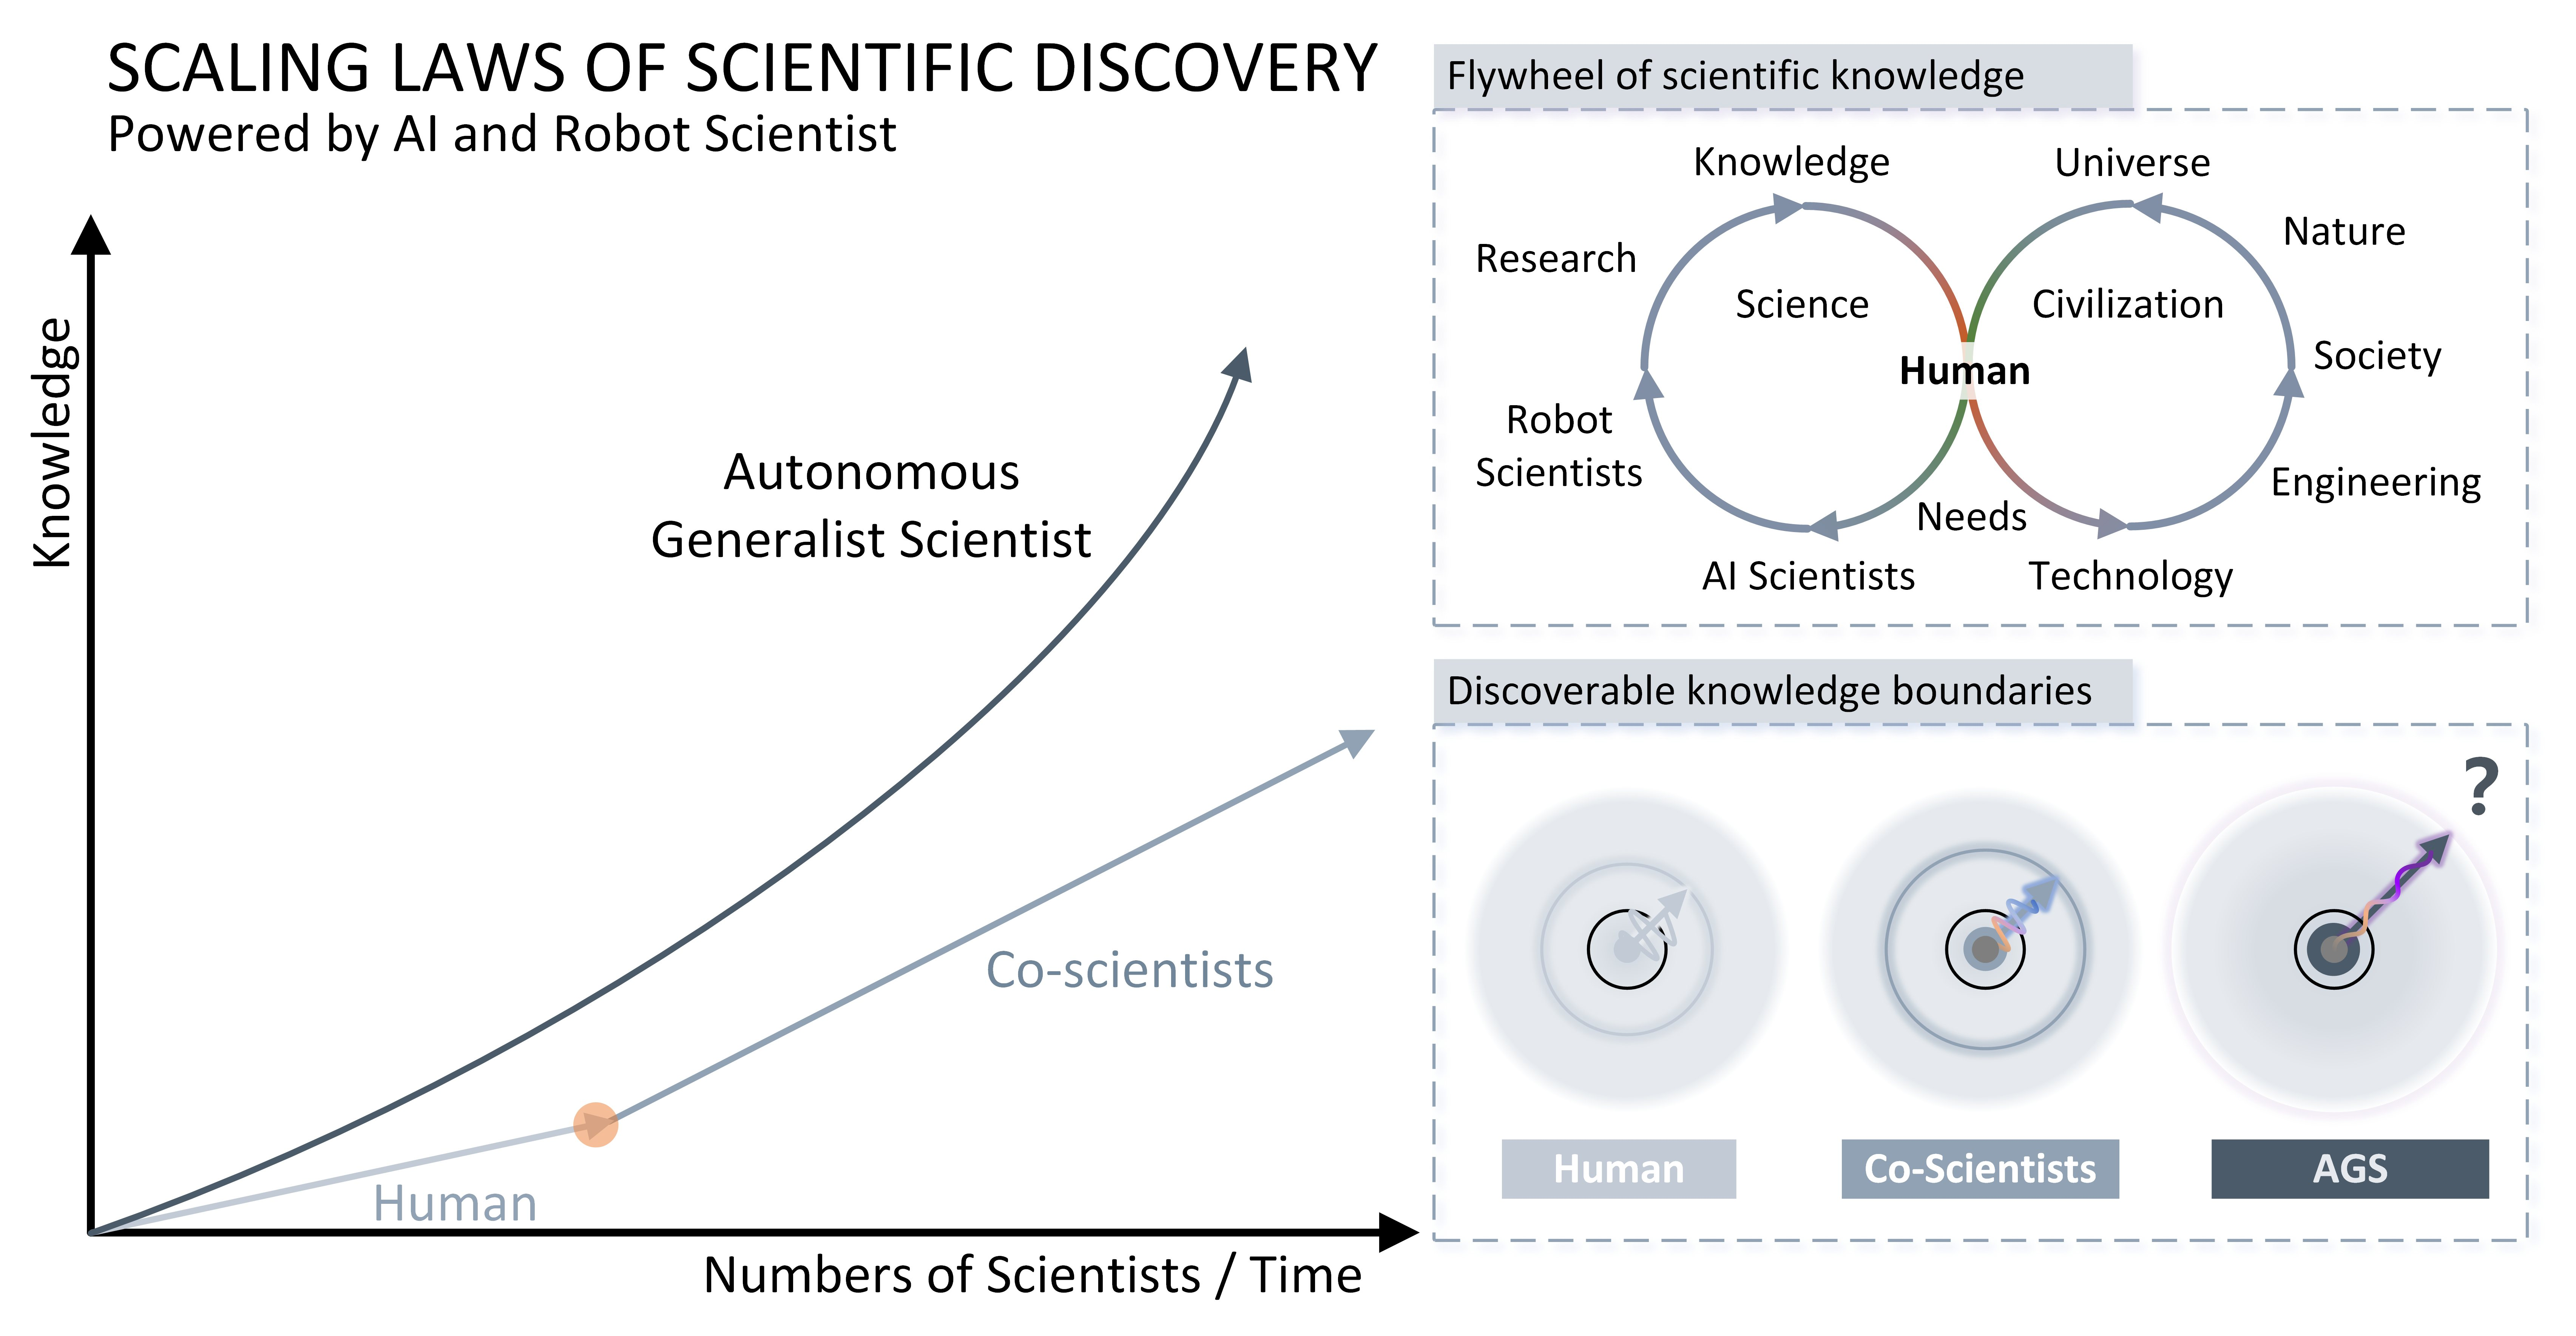
\includegraphics[width=1.00\columnwidth]{resources/figures/ags_paradigm.jpg}}
\caption{Evolution of scientific discovery paradigms: from human-centered research through collaborative systems to autonomous generalist scientists- breaking and transcending physical and knowledge boundaries.}
\label{ags_paradigm}
\end{center}
\vskip -0.2in
\end{figure}




\begin{figure}[ht]
\vskip 0.2in
\begin{center}
\centerline{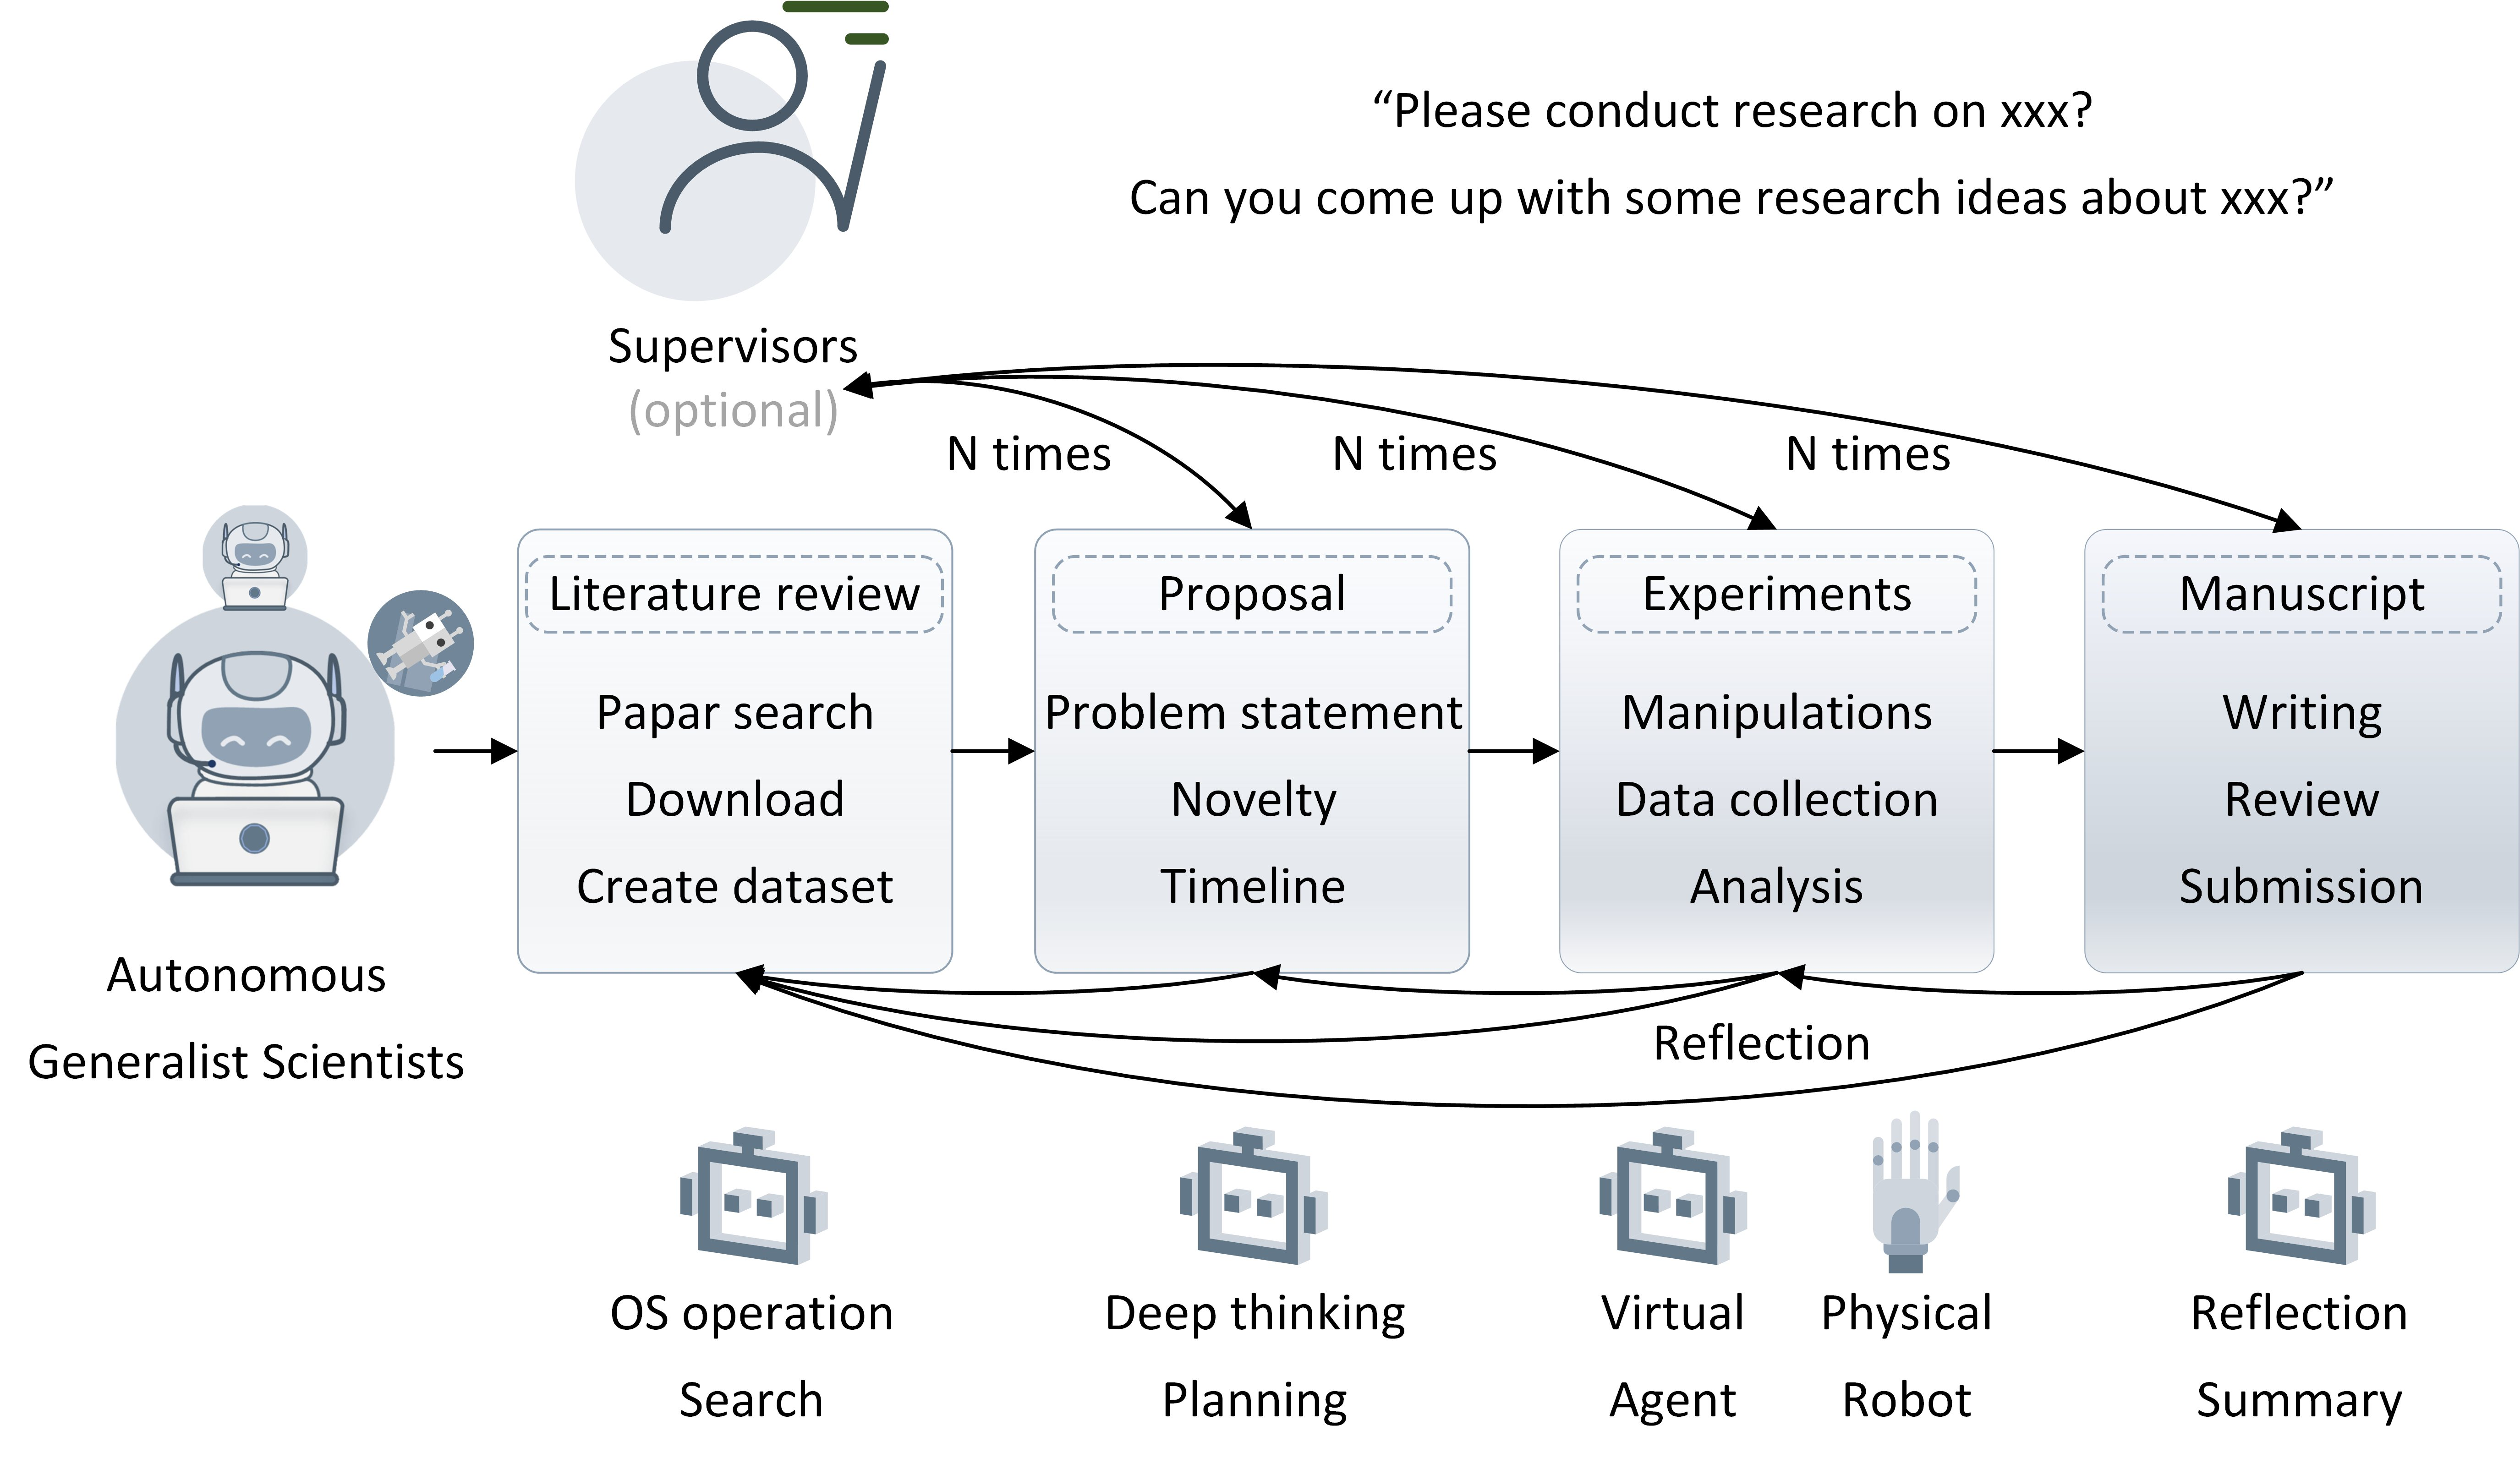
\includegraphics[width=1.00\columnwidth]{resources/figures/ags_framework.jpg}}
\caption{Framework of autonomous generalist scientist based on AI agents and robots. Research agent/robot can accelerate scientific research progress and bridge the gap between scientific knowledge in different disciplines.}
\label{ags_framework}
\end{center}
\vskip -0.2in
\end{figure}
